\documentclass{article}
\usepackage{amsthm, amsmath, listings, graphicx}
\usepackage[margin=0.5in]{geometry}
\graphicspath{ {hw3_img/} }

\begin{document}
    \noindent\textbf{CS 375 Homework 1}\hfill Anchu A. Lee\\
    \noindent\today
    \\\\“I have done this assignment completely on my own. I have not copied it, nor have I given my solution to anyone else. I understand that if I am involved in plagiarism or cheating I will have to sign an official form that I have cheated and that this form will be stored in my official university record. I also understand that I will receive a grade of 0 for the involved assignment for my first offense and that I will receive a grade of “F” for the course for any additional offense.” 
    \\\\
    \begin{enumerate}
        \item Suppose the capacity of the knapsack is 30 and the set of items 
        $S = \{(item_1, 5, \$50)$, $(item_2, 20, \$140)$, $(item_3, 10, \$60)$, 
        $(item_4, 10, \$80)\}$ where each element of set S represents (item, 
        weight, profit). Find an optimal solution for the fractional knapsack 
        problem using the greedy algorithm introduced in class. Show both the 
        order in which the items are selected and the optimal solution you 
        find.\\\\
            \begin{tabular}{| c || c | c | c | c |}
                \hline
                Item & $item_1$ & $item_4$ & $item_2$ & $item_3$ \\
                \hline
                Profit & $50$ & $80$ & $140$ & $60$ \\ 
                \hline
                Weight & $5$ & $10$ & $20$ & $10$ \\
                \hline
                Value & $10$ & $8$ & $7$ & $6$ \\
                \hline
            \end{tabular}
        \item Find a longest common subsequence (LCS) between two strings 
        $X = APPLE$ and $Y = PLATE$ using the dynamic programming algorithm 
        discussed in class. Provide your solution steps in a table that 
        includes the solutions for all possible subproblems and directed 
        arrows (diagonal, left, and up arrows) needed to find an LCS in the 
        end. Use the recursive method discussed in class to find an LCS based 
        on the information stored in the table. Note: show both an LCS and the 
        path that leads to the LCS.
        \item Briefly describe how to extend the depth first search (DFS) 
        algorithm introduced in the class to determine whether a directed 
        graph has a cycle (You may give a sketch of pseudo code and highlight 
        the lines that are different from the original DFS algorithm. Comment 
        your pseudo code to make it easy to understand).
        \item In graph theory, a connected component of an undirected graph is 
        a subgraph in which any two vertices are reachable to each other 
        (i.e., connected by at least one path), but the subgraph is not 
        connected to any additional vertices in the supergraph. Briefly 
        describe how to extend the breadth first search (BFS) algorithm 
        introduced in the class to determine the number of connected 
        components in an undirected graph (You may give a sketch of pseudo 
        code and highlight the lines that are different from the original BFS 
        algorithm. Comment your pseudo code to make it easy to understand).
        \item Enumerate the nodes in the following graph in (a) BFS order and 
        (b) DFS order, starting from node 1. 
            \begin{center}
                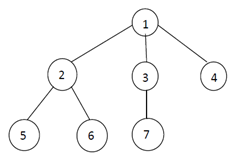
\includegraphics{tree1}
            \end{center}
        \item For each node $u$ in an undirected graph $G(V, E)$, let 
        $sDegree(u)$ be the sum of the degrees of the neighbors of $u$, that 
        is, $sDegree(u) = \sum_{(u,v)\in E}Degree(v)$. Given an adjacency-list 
        implementation of a graph $G(V, E)$, provide pseudo code (comment your 
        pseudo code to make it easy to understand) for an $O(|V|+|E|)$ 
        algorithm that outputs for each node $u$ its $sDegree(u)$, and briefly 
        analyze the time complexity of your algorithm to justify it is 
        $O(|V|+|E|)$.
        \item Consider a modification to the activity selection problem in 
        which each activity $a_i$ has, in addition to a start and finish time, 
        a value $v_i$. The objective is no longer to maximize the number of 
        compatible activities scheduled, but instead to maximize the total 
        value of the compatible activities scheduled. This is called the 
        weighted activity selection problem. Develop a bottom-up dynamic 
        programming solution for this problem. Your solution should have a 
        time complexity in $O(n^2)$, where n is the total number of activities 
        in the input.
    \end{enumerate}
\end{document}